\mychapter{vision}{Vision, concepts and principles}
\begin{figure}
  \begin{center}
    \centerline{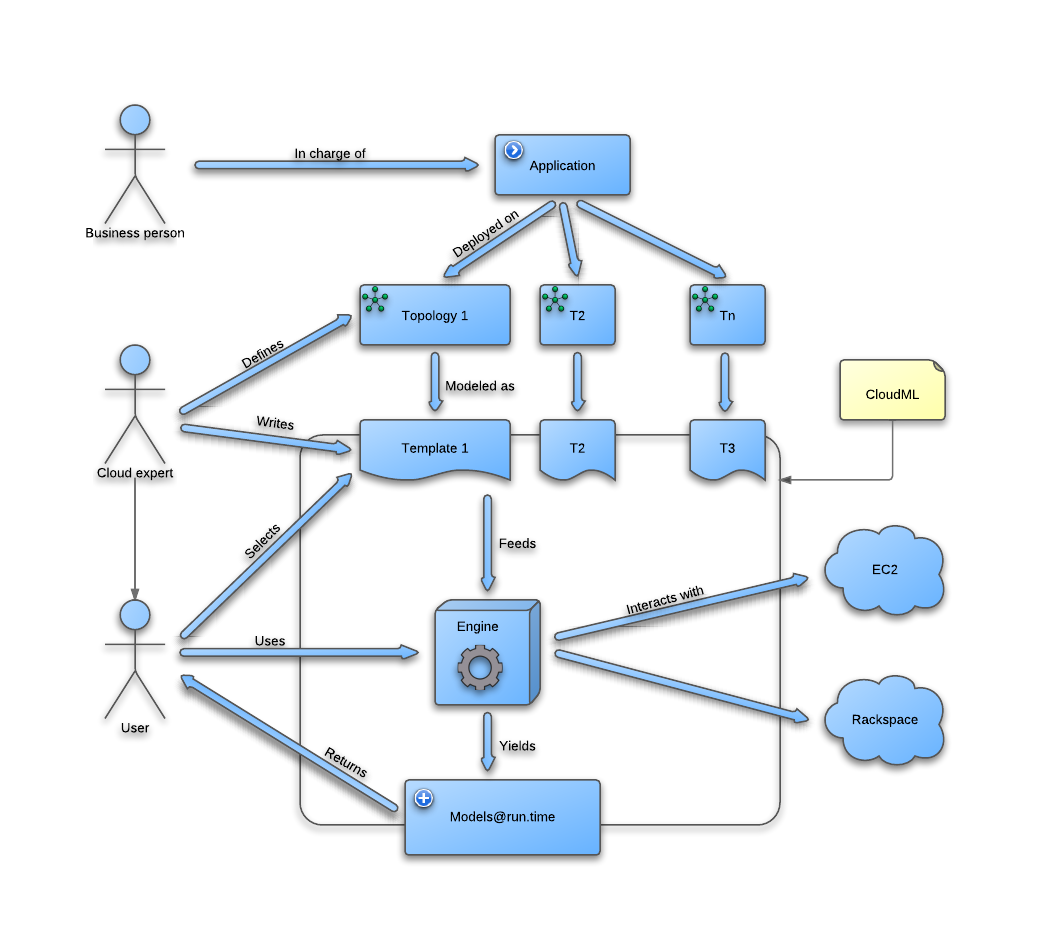
\includegraphics[width=1.5\linewidth]{img/big-picture.png}}
    \caption{``Big picture'', overview of CloudML procedure flow.}
    \label{fig:big-picture}
  \end{center}
\end{figure}


In this chapter the core idea of CloudML will be presented.
The concept and principle of CloudML is to be an easier and more reliable
path into cloud computing for IT-driven businesses of variable sizes.
The tool is visioned to parse and execute template files representing topologies
and provision these as instances available in the cloud. 

The vision of CloudML is reflected through \citefig{big-picture} which gives
an overview of the procedure flow in and around CloudML.

\paragraph{Domain of CloudML.}

Inside \citefig{big-picture} there is an area pointed out as \emph{CloudML},
this area contain components necessary to implement in order to fulfill
the vision as a whole.
Every part within the designated area is some physical aspect in the 
implementation, and therefore core parts of the contribution.

\paragraph{The actors.}

In \citefig{big-picture} there are three actors,
\begin{ii}
  \iitem business person representing someone with administration- or manager position which
    defines and controls demands for application functionality and capabilities.
    The next actor,
  \iitem cloud expert has a greater knowledge of the cloud domain 
    \eg cloud providers,
    services these offer, limitations, API support and prices.
    The last actor,
  \iitem user is a person which directly utilize CloudML to do provisioning.
    This physical person may or may not have the role of cloud expert, 
    hence the cloud expert extends from the user actor.
\end{ii}

\paragraph{Application and topologies.}

The business person is in charge of the application, he/she has a need
for an application that can fulfill certain tasks, and to handle these 
tasks application demands are made.
The cloud expert use the requirements sketched by the business person to 
define and design node topologies which tackles the application demands.
A topology is a map of nodes connected together in a specific pattern, 
defined by the cloud expert.
In a topology there is also information about node attributes 
\eg \myac{CPU} power and \myac{RAM} sizes.
He/she might create several topologies to fulfill the application demands.

\paragraph{Templates.}

The next step is to create templates based on the topologies, this is done by
the cloud expert.
A template is a digital reflection of a topology including the attributes and some additional 
information such as node names and template labeling.
It is also possible to define more than one topology within a single template.

\paragraph{Engine.}

When the cloud expert have designed and created the necessary templates the next actor, 
user, will continue the procedure.
The user selects the template and feeds them into the engine.
The engine is the core of the implementation, handling several steps and executing
most of the CloudML logic.
The engine operates according to five different steps:
\begin{enumerate}
  \item Convert the template files into a native format for later use.
  \item Convert pure nodes into instances ready for provisioning.
  \item Connect to all the desired providers.
  \item Propagate the instances.
  \item Produce models@run.time of the instances being propagated.
\end{enumerate}

\paragraph{Providers.}

The engine interacts with the providers, in \citefig{big-picture} 
\myac{EC2} and Rackspace are selected as examples, but any
cloud provider that will be supported by CloudML can be utilized.
As discussed in \citechap{state-of-the-art} and \citechap{challenges}
different providers implement different solutions for communication
\eg for provisioning nodes, managing nodes and services or terminating instances.
For the engine to interact with a set of different providers, 
a tool, library or framework is needed.
This additional software can connect to the different providers through a common interface.

\paragraph{Models@run.time.}

The last part of this implementation of CloudML (see \citechap{perspectives}) is to
reflect provisioned instances with models@run.time.
These models are returned to the user when provisioning starts, 
and when attributes and statuses about instances are updated the user is 
notified about these updates through the models.
In the implementation the models can extend from or aggregate \emph{instances}.
